\documentclass{article}
\usepackage{graphicx}
\usepackage{amsmath}
\usepackage{amssymb}
\usepackage{natbib}
\renewcommand{\refname}{References}
\usepackage{url}

\title{On Trading of ETFs based on the Differential Geometric Forecast Model}

\author{Babak Emami}

\date{\today}

\begin{document}
\maketitle

\begin{abstract}


\end{abstract}

\section{Introduction}\label{section:introduction}

Here we propose two approaches for trading of exchanged-traded
funds (ETFs) based on the differential geometric economic forecast
model. The reader should refer to the notes on this model for details.

\section{Approach I: Maximize Predicted Return}\label{section:approach-1}

The first proposed approach is based on maximization of predicted
portfolio value growth normalized by standard deviation of prediction,
that is the risk associated with forecast. This approach is in theory
reasonable. However, as will be shown, this approach does not work
because the model is not accurate enough. As we improve the model,
this approach may become relevant.

At any given current time $t_{0}$ we build a differential geometric
model based on historical data. The model consists of $n$ economic
variable including $\tilde{n}$ ETFs that we plan to use for trading.

The model provides us with a system of ODEs; given the current values
of the model's $n$ economic variables as initial conditions, the
solution of these ODEs yields forecast of economic variables.

Let us assume that we entered $q_{i}$ positions of asset $i$ at time
$t_{0}$; the values are posive and negative for long and short
positions, respectively. The predicted value of our portfolio at time
$t$ > $t_{0}$, that is $V(t)$ is calculated as,

\begin{equation}\label{eqn:prt-value}
V(t) = \sum_{i=1}^{\tilde{n}} q_{i} y^{i}(t)
\end{equation}

where $y^{i}(t)$ is predicted price of asset $i$ at time $t$. 

Note that we consider $y^{i}(t)$ a random variable with an expected
value of $\bar{y}^{i}(t)$ and a standard deviation of $\sigma^{i}$ (it
is not a function of time). The expected portfolio value is calculated
as

\begin{equation}\label{eqn:expected-prt-value}
\bar{V}(t) = \sum_{i=1}^{\tilde{n}} q_{i} \bar{y}^{i}(t)
\end{equation}

The variance of $V(t)$ is calculated as

\begin{equation}\label{eqn:stdev-prt-value}
Var(V(t)) = \sum_{i=1}^{\tilde{n}} q_{i}^{2} (\sigma^{i})^{2}
\end{equation}

We determine the asset quantities $q_{i}$ by solving the following
optimization problem,

\begin{equation}\label{eqn:optimization-problem-V}
\max_{q_{i}} \frac{\bar{V}(t_{H})-V(t_{0})}{\[Var(V(t_{H})-V(t_{0})\]}
\end{equation}

Using Eqs.~\ref{eqn:expected-prt-value} and \ref{eqn:stdev-prt-value},
we get

\begin{equation}\label{eqn:optimization-problem-q}
\max_{q_{i}} \frac{\sum_{i=1}^{\tilde{n}}
  q_{i} \[\bar{y}^{i}(t_{H})-y^{i}(t_{0})\]}{\[\sum_{i=1}^{\tilde{n}}
  q_{i}^{2} (\sigma^{i})^{2}\]^{1/2}}
\end{equation}

where $t_{H}$ > $t_{0}$ is the end of our trading horizon. In other
words, we plan to adjust our portfolio again at $t{H}$, or more
generally every $t_{H}-t{0}$.

When solving \ref{eqn:optimization-problem-q}, we should consider that
values of $q^{i}$ can be only integers. A simpler approach is to
convert quantities to portfolio weights; $w_{i} = \frac{q_{i}
  y^{i}(t_{0})}{V(t_{0})}$. The optimization probelm become,

\begin{equation}\label{eqn:optimization-problem-w}
\max_{w_{i}} \frac{\sum_{i=1}^{\tilde{n}}
  w_{i} r^{i}(t_{H})}{\[\sum_{i=1}^{\tilde{n}}
  w_{i}^{2} \(\frac{\sigma^{i}}{y^{i}(t_{0})\)^{2}\]^{1/2}}
\end{equation}

subject to the following equality constraint,

\begin{equation}\label{eqn:sum-constraint}
\sum_{i=1}^{\tilde{n}} |w_{i}| = 1
\end{equation}

where $r^{i}(t) = \frac{\bar{y}^{i}(t)-y^{i}(t_{0})}{y^{i}(t_{0})}$ is
the expected return on asset $i$.

For short trading horizons, for example a day, the standard deviation
of model forecasts are rather high and overwhelm the actual price
movements. As such, the above algorithm does not work. We tested the
above agolrithm using a differential geometric consisting of 27 ETFs
and 7 continuous futures contracts, that is a total of 34 economic
variables; the 27 ETFs were used as portfolio assets.

\begin{figure}
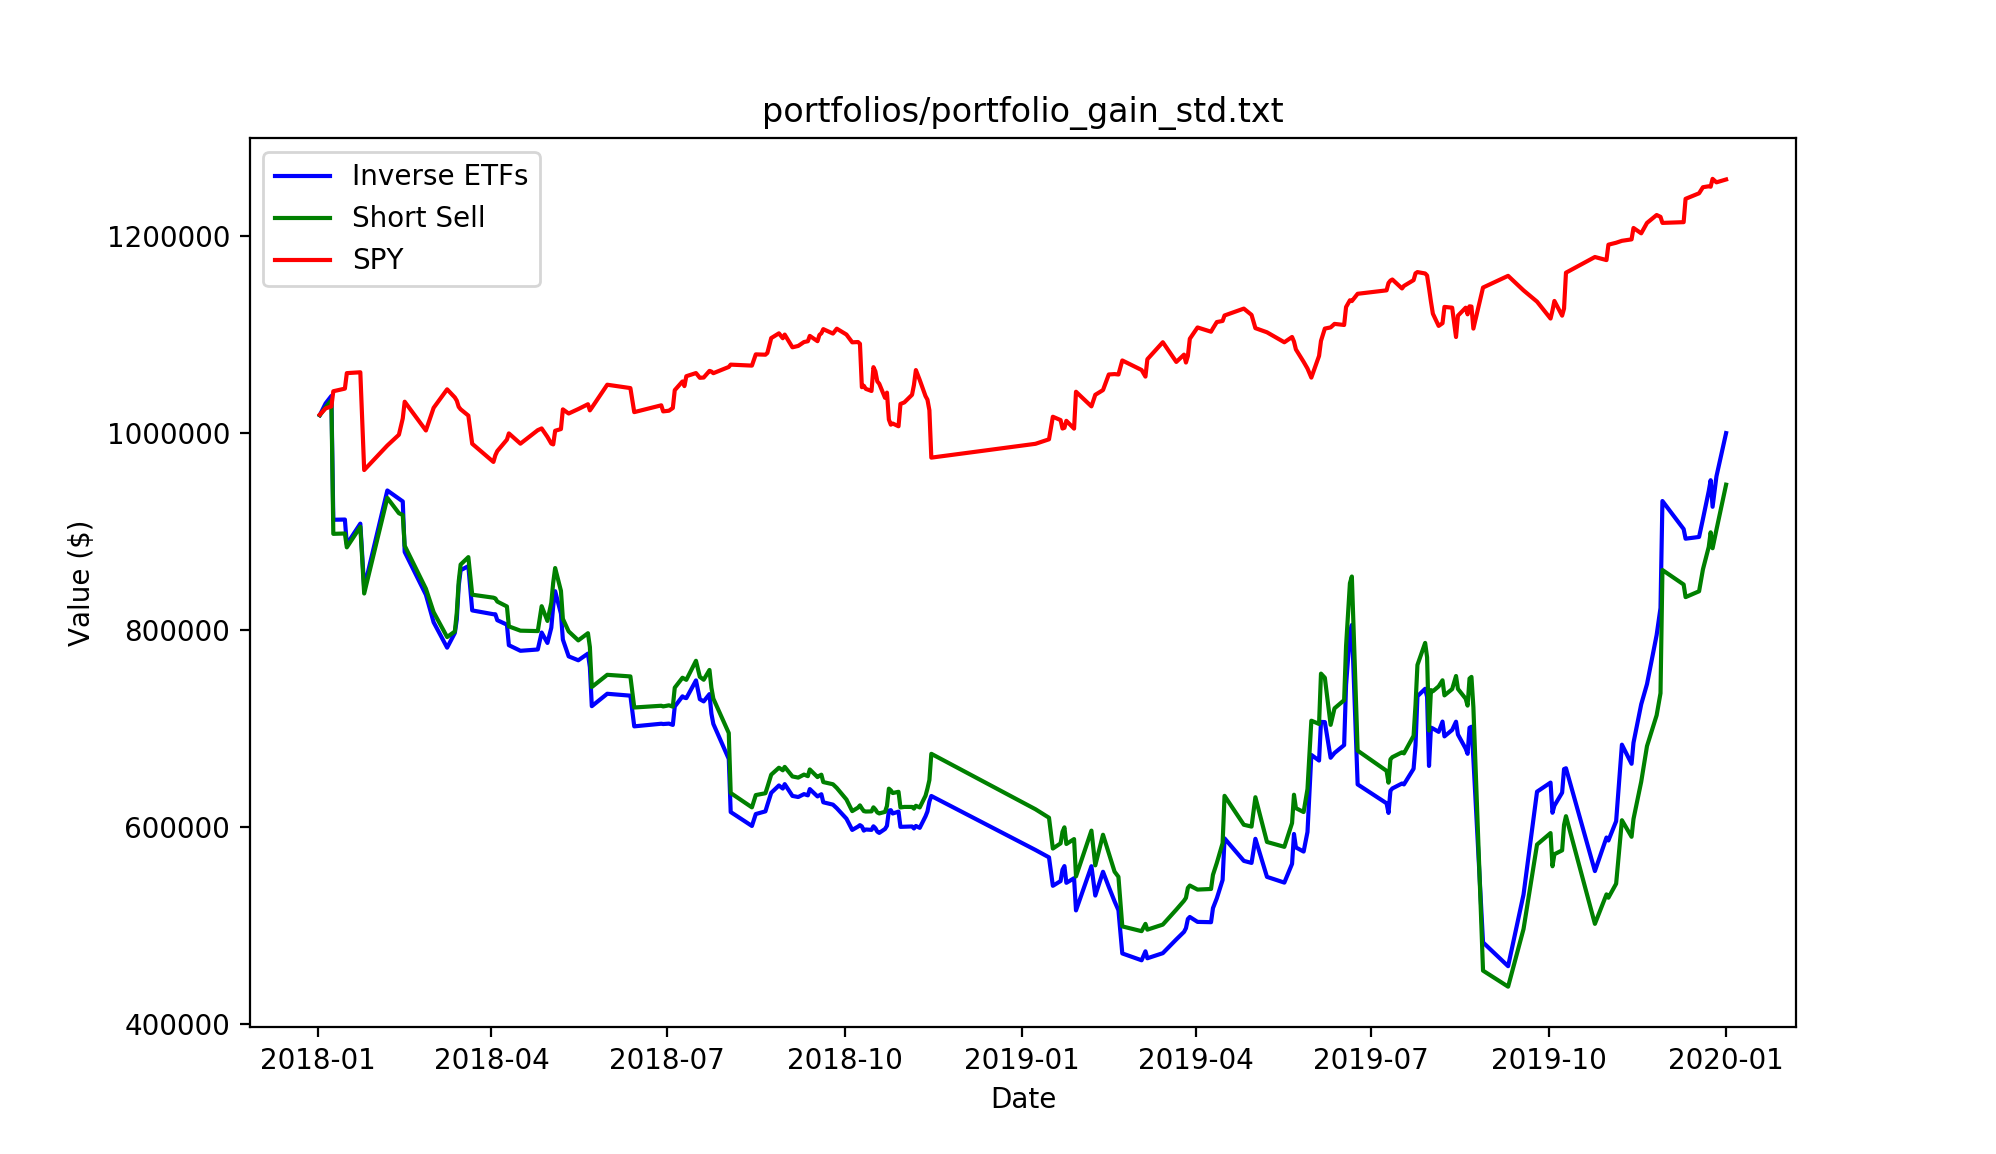
\includegraphics[scale=0.42,bb=0 0 320 240]{figures/Gain_std_maximization.png}
\caption{Results of ETF trading backtest using approach I; portfolio
  gain to standard deviation ratio.}
\label{fig:etf-results-approach-1}
\end{figure}

\section{Approach II: Historical Return and MAD}\label{section:approach-2}






A trading algorithm which uses the above-mentioned differential
geometric model to forecast price of securities. In a nutshell, given
a pool of securities, we propose building a portfolio by minimizing
mean absolute deviation (MAD) where taking a long or short position on
each security is based on the price trend as predicted by the manifold
model.

Let us us assume that we trade with a pool of $\tilde{n}$ assets with
return of logs $X_{i}(t)$, where $i = 1, ...,\tilde{n}$. Note that
$X_{i}(t) = \frac{\log(P_{i}(t))
  -\log(P_{i}(t-1))}{\log(P_{i}(t-1))}$, where $P_{i}$ is price of
asset $i$. The proposed trading algorithm is in fact solving the
following constrained optimization problem,

\begin{equation}\label{eqn:mad-optimization-problem}
\min_{w_{i}} \frac{1}{\tilde{N}}\sum_{t=t_{curr}}^{t_{curr}-\tilde{N}+1}
|\sum_{i=1}^{\tilde{n}} w_{i} (X_{i}(t)-\bar{X_{i}})|
\end{equation}

subject to equality constraint

\begin{equation}\label{eqn:mad-sum-constraint}
\sum_{i=1}^{\tilde{n}} |w_{i}| = 1
\end{equation}

and inequality constraint

\[
\begin{cases}\label{eqn:mad-trend-constraint}
    w_{i} > 0 & \text{if upward forecast price trend} \\
    w_{i} < 0 & \text{if downward forecast price trend}
\end{cases}
\]

where $w_{i}$ is the portfolio weight for asset $i$; a positive or
negative weight indicates a long or short position, respectively. Also
note that $\tilde{N}$ indicates the number of data points used for
calculation of MAD, i.e. $t_{k} \in [\tilde{T},T]$ where $k = 1,
...,\tilde{N}$.

\subsection{A Fallback Plan for Trend Prediction}\label{subsection:fallback-macd}

It is advised to keep a short out-of-sample period with available
historical data for each forecast model. We can then test the
performance of the model's trend prediction for each asset. If a model
fails to predict the correct trend of a security price in the
out-of-sample period following the training period, it will likely
fail beyond the out-of-sample period as well. In this case, we can
fall back on one of the more standard trend prediction
methodologies. As an example, we can use Moving Average Convergence
Divergence (MACD) method.

MACD is used to calculate short term acceleration of a security and as
such helps with making a decision to take a long or short position on
a security. MACD of a signal $x(t)$ is defined as,

\begin{equation}\label{eqn:macd}
F_{MACD}^{(f,s)}(x)|_{t_{curr}} = E^{f}(x)|_{t_{curr}} -
E^{s}(x)|_{t_{curr}}
\end{equation}

where $E^{p}$ represents exponential moving average with respect to a
period $p$, and $f$ and $s$ are fast and slow periods,
respectively. The signal $x(t)$ has a positive/negative acceleration
at $t=t_{curr}$ if $F_{MACD}^{(f,s)}(x)|_{t_{curr}}$ is
greater/smaller than $E^{r}(F_{MACD}^{(f,s)}(x))|_{t_{curr}}$, where
$r$ is called the signal period. The standard values for fast, slow,
and signal periods are 12, 26, and 9 days, respectively. One should
long/short when acceleration becomes positive/negative. In fact, one
can check the sign of both $F_{MACD}^{(f,s)}(x)|_{t_{curr}}$ and
$F_{MACD}^{(f,s)}(x)|_{t_{curr}}-E^{r}(F_{MACD}^{(f,s)}(x))|_{t_{curr}}$
as they represent velocity and acceleration signs, respectively. The
number of historical times used to calculate MACD should be at least
$s$ + $r$ ($N > s + r$).

\subsection{Some Trading Backtest Results}\label{subsection:trading-backtest}

The proposed trading algorithm was backtested over a number of recent
years. Here we have used a pool of 11 ETFs for trading,

\begin{itemize}
    \item[] QQQ: PowerShares QQQ 
    \item[] SPY: SPDR S\&P 500 Growth ETF 
    \item[] DIA: SPDR Dow Jones Industrial Average ETF 
    \item[] MDY: SPDR S\&P MidCap 400 ETF 
    \item[] IWM: iShares Russell 2000 Index Fund 
    \item[] OIH: Market Vectors Oil Services ETF 
    \item[] SMH: Market Vectors Semiconductor ETF 
    \item[] XLE: Energy Select Sector SPDR Fund 
    \item[] XLF: Financial Select Sector SPDR Fund 
    \item[] XLU: Utilities Select Sector SPDR Fund 
    \item[] EWJ: iShares MSCI Japan Index Fund
\end{itemize}

The models and portfolio weights were generated at the beginning of
each business day and the portfolio was adjusted using the updated
weights on a daily basis. For each ''current'' date, the previous 360
days were used, where the first 357 days was used for training and the
last three days was kept as the out-of-sample period; MACD was used as
a fallback strategy whenever the model failed to predict the trend in
the out-of-sample period. We used Quantioan~\cite{ref:quantopian} to
run backtests and generate plots.

Figure~\ref{fig:backtest-2019-half} shows the backtest results of the
proposed algorithm for the first half of 2019 (blue line), compared to
performance of SPY (red line). As can be seen, the proposed algorithm
shows a better performance.

A similar trend is observed in the backtest results going back to
2012, as can be seen in Figures~\ref{fig:backtest-2018} to
~\ref{fig:backtest-2012}. The only exception is 2016, where the
proposed algorithm is superior to SPY in the first quarter, however,
performs poorly for the rest of 2016. The performance is also poor in
the first 4 months of 2012.

Figure~\ref{fig:backtest-2007-2008} shows backtest results for
2007-2008 period. This is specifically of interest, because this
period shows the performance of the algorithm during the 2008 economic
crisis. As can be seen, the algorithm certainly performs better than
SPY. While these results may not be realistic, as the market may not
be liquid enough for taking short positions on losing assets during an
economic crisis, it is likely that using this algorithm could have
protected portfolios that were built based on it.

\subsection{Trading Algorithm Parameter Study}\label{subsection:mad-parameter-study}

We performed a study on the effect of the period used for calculation
of MAD, $\tilde{N}$ in Eq.~\ref{eqn:mad-optimization-problem}.

\newpage

\begin{figure}
\includegraphics[scale=0.42,bb=0 0 320 240]{figures/results-SPY.png}
\caption{In-sample and out-of-sample forecast results for SPY.}
\label{fig:results-spy}
\end{figure}

\begin{figure}
\includegraphics[scale=0.9,bb=0 0 640 480]{figures/results-SPY-oos.png}
\caption{Out-of-sample forecast results for SPY.}
\label{fig:results-spy-oos}
\end{figure}

\begin{figure}
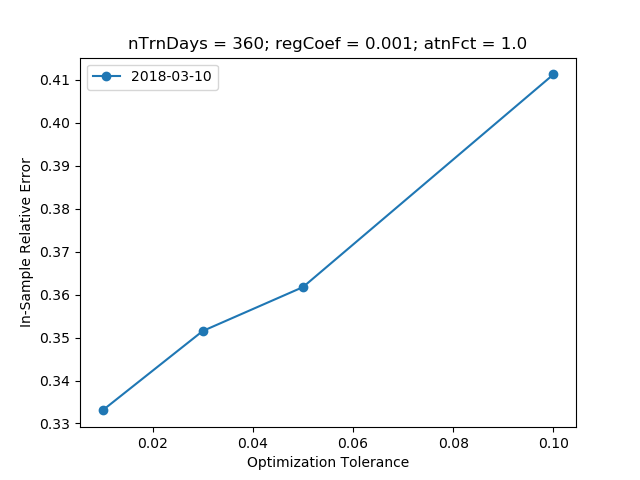
\includegraphics[scale=0.9,bb=0 0 640 480]{figures/tolerance-sensitivity-error.png}
\caption{In-sample relative error vs. optimization tolerance; $T$ =
  360 days, $\eta(t) = 1.0$, $\zeta$ = 1.0e-3.}
\label{fig:tolerance-sensitivity-error}
\end{figure}

\begin{figure}
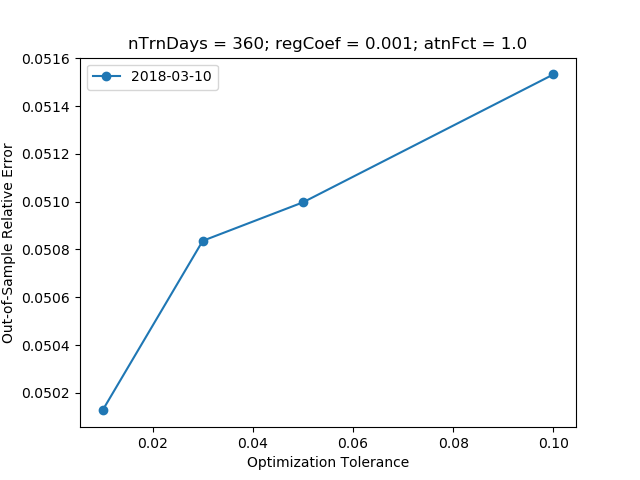
\includegraphics[scale=0.9,bb=0 0 640 480]{figures/tolerance-sensitivity-oos-error.png}
\caption{Out-of-sample relative error vs. optimization tolerance; $T$
  = 360 days, $T^{oos}$ = 3, days$\eta(t)$ = 1.0, $\zeta$ = 1.0e-3.}
\label{fig:tolerance-sensitivity-oos-error}
\end{figure}

\begin{figure}
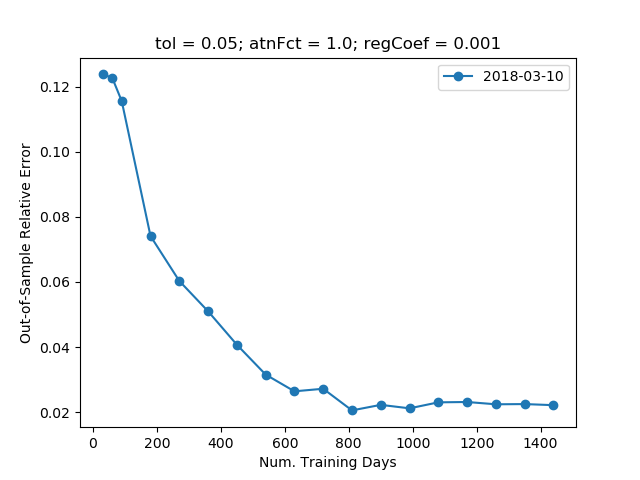
\includegraphics[scale=0.9,bb=0 0 640 480]{figures/nTrnDays-sensitivity-oos-error.png}
\caption{Out-of-sample relative error vs. number of days used for
  training; $T^{oos}$ = 3, $\eta(t)$ = 1.0, $\zeta$ = 1.0e-3,
  tolerance = 0.05.}
\label{fig:nTrnDays-sensitivity-oos-error}
\end{figure}

\begin{figure}
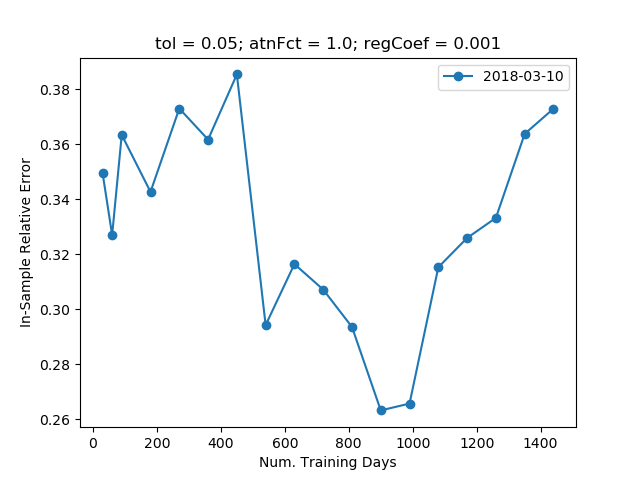
\includegraphics[scale=0.9,bb=0 0 640 480]{figures/nTrnDays-sensitivity-error.png}
\caption{In-sample relative error vs. number of days used for
  training; $\eta(t) = 1.0$, $\zeta$ = 1.0e-3, tolerance = 0.05.}
\label{fig:nTrnDays-sensitivity-error}
\end{figure}

\begin{figure}
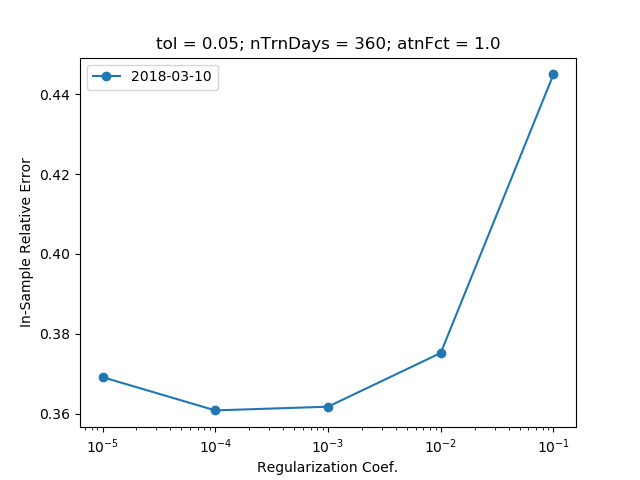
\includegraphics[scale=0.9,bb=0 0 640 480]{figures/regCoef-sensitivity-error.png}
\caption{In-sample relative error vs. regularization coefficient; $T$
  = 360 days, $\eta(t)$ = 1.0, tolerance = 0.05.}
\label{fig:regCoef-sensitivity-error}
\end{figure}

\begin{figure}
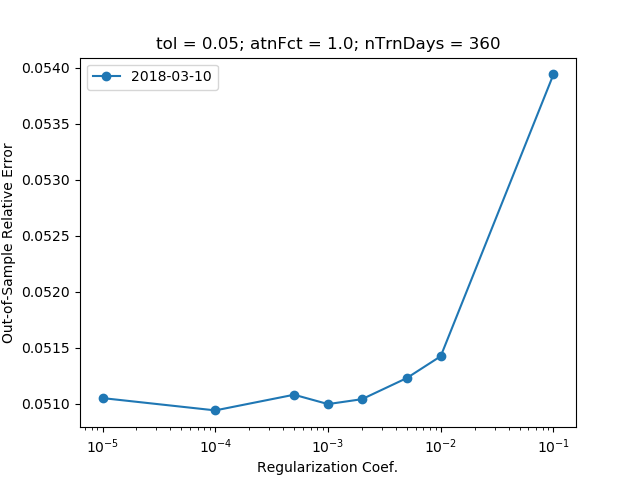
\includegraphics[scale=0.9,bb=0 0 640 480]{figures/regCoef-sensitivity-oos-error.png}
\caption{Out-of-sample relative error vs. regularization coefficient;
  $T$ = 360 days, $T^{oos}$ = 3, $\eta(t)$ = 1.0, tolerance = 0.05.}
\label{fig:regCoef-sensitivity-oos-error}
\end{figure}

\begin{figure}
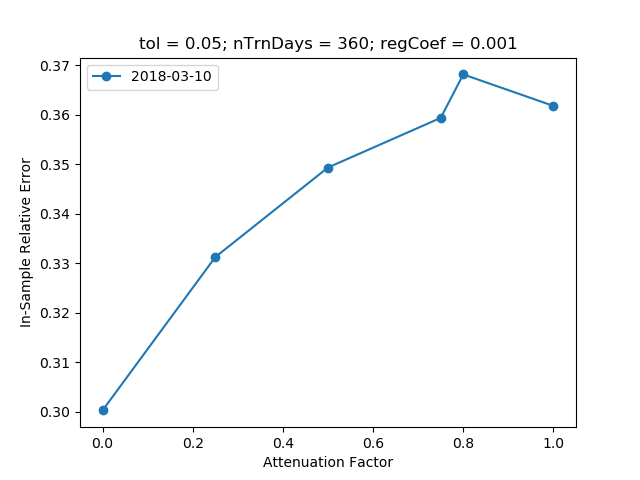
\includegraphics[scale=0.9,bb=0 0 640 480]{figures/atnFct-sensitivity-error.png}
\caption{In-sample relative error vs. attenuation parameter; $T$ = 360
  days, $\zeta$ = 1.0e-3, tolerance = 0.05.}
\label{fig:atnFct-sensitivity-error}
\end{figure}

\begin{figure}
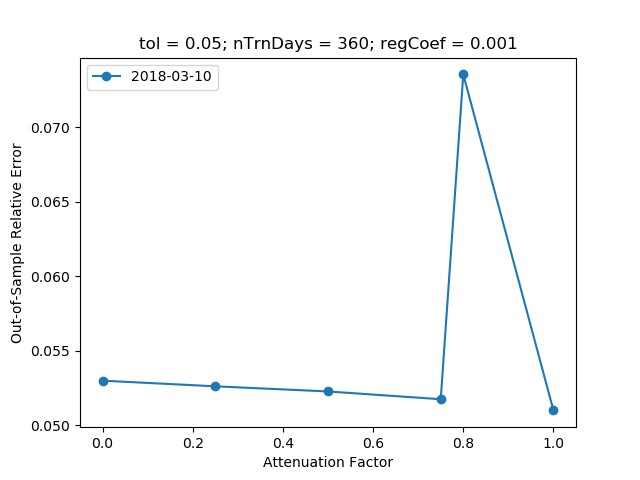
\includegraphics[scale=0.9,bb=0 0 640 480]{figures/atnFct-sensitivity-oos-error.png}
\caption{Out-of-sample relative error vs. attenuation parameter; $T$ =
  360 days, $T^{oos}$ = 3, $\zeta$ = 1.0e-3, tolerance = 0.05.}
\label{fig:atnFct-sensitivity-oos-error}
\end{figure}

\begin{figure}
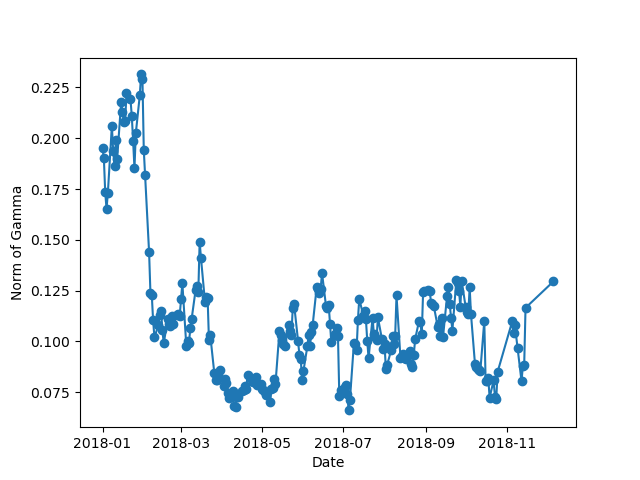
\includegraphics[scale=0.9,bb=0 0 640 480]{figures/Gamma_time_2018.png}
\caption{Norm of Gamma vs. snapdate Each point on the plot comes from
  a model with a constant Christoffel symbol; for all models we have
  $T$ = 360 days, $\zeta$ = 1.0e-3, $\eta_{0}$ = 1.0, tolerance =
  0.05.}
\label{fig:gamma-time}
\end{figure}

\begin{figure}
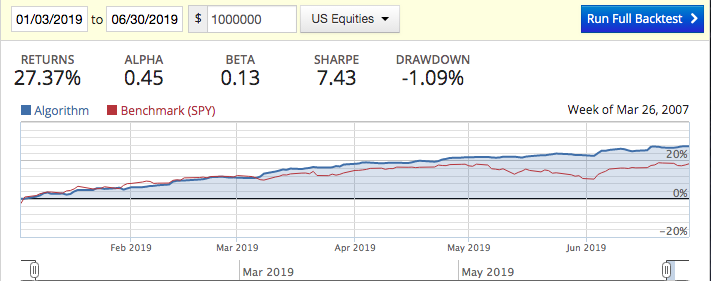
\includegraphics[scale=0.5,bb=0 0 640 480]{figures/2019_half_mfd_macd.png}
\caption{Comparison of proposed algorithm (blue) to SPY (red); first
  half of 2019.}
\label{fig:backtest-2019-half}
\end{figure}

\begin{figure}
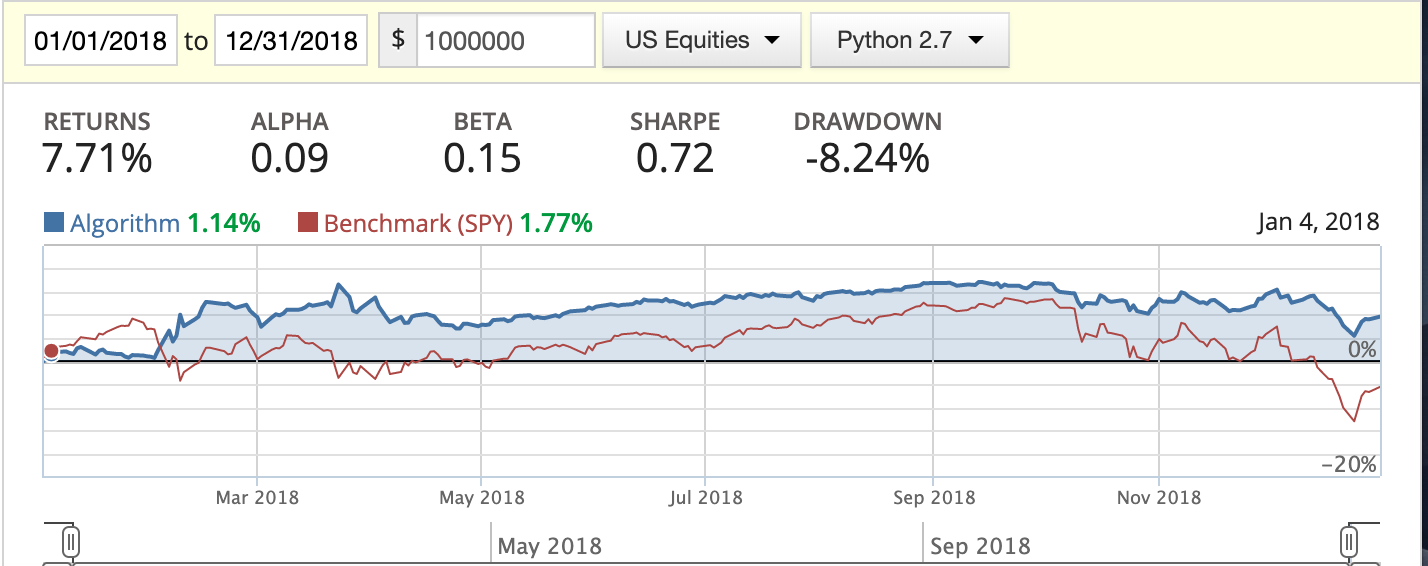
\includegraphics[scale=0.5,bb=0 0 640 480]{figures/mad_mfd_macd_2018.png}
\caption{Comparison of proposed algorithm (blue) to SPY (red); 2018.}
\label{fig:backtest-2018}
\end{figure}

\begin{figure}
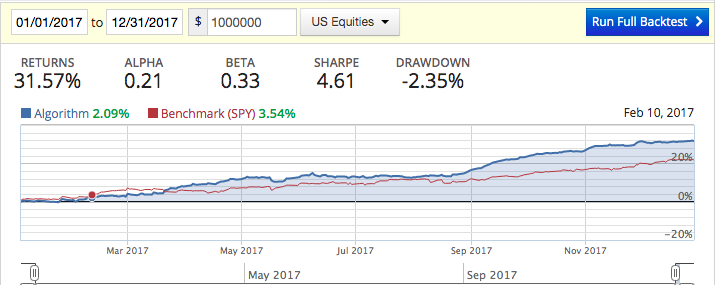
\includegraphics[scale=0.5,bb=0 0 640 480]{figures/mad_mfd_macd_2017.png}
\caption{Comparison of proposed algorithm to SPY; 2017.}
\label{fig:backtest-2017}
\end{figure}

\begin{figure}
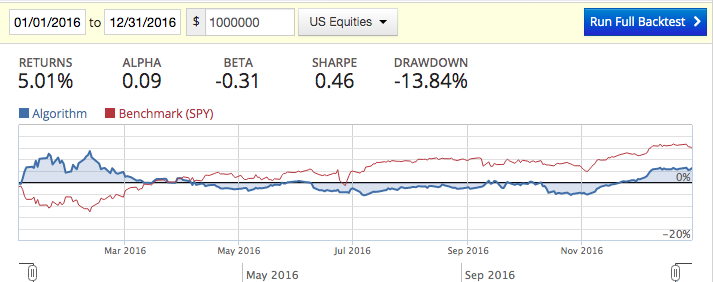
\includegraphics[scale=0.5,bb=0 0 640 480]{figures/mad_mfd_macd_2016.png}
\caption{Comparison of proposed algorithm to SPY; 2016.}
\label{fig:backtest-2016}
\end{figure}

\begin{figure}
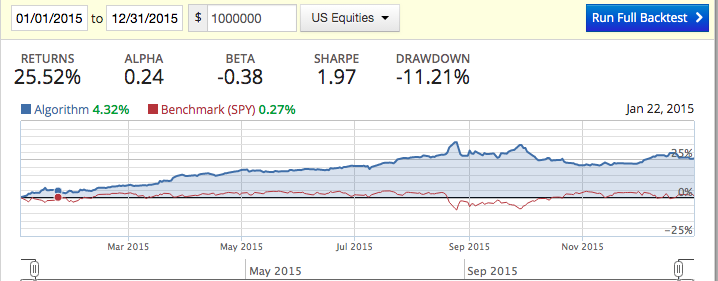
\includegraphics[scale=0.5,bb=0 0 640 480]{figures/mad_mfd_macd_2015.png}
\caption{Comparison of proposed algorithm to SPY; 2015.}
\label{fig:backtest-2015}
\end{figure}

\begin{figure}
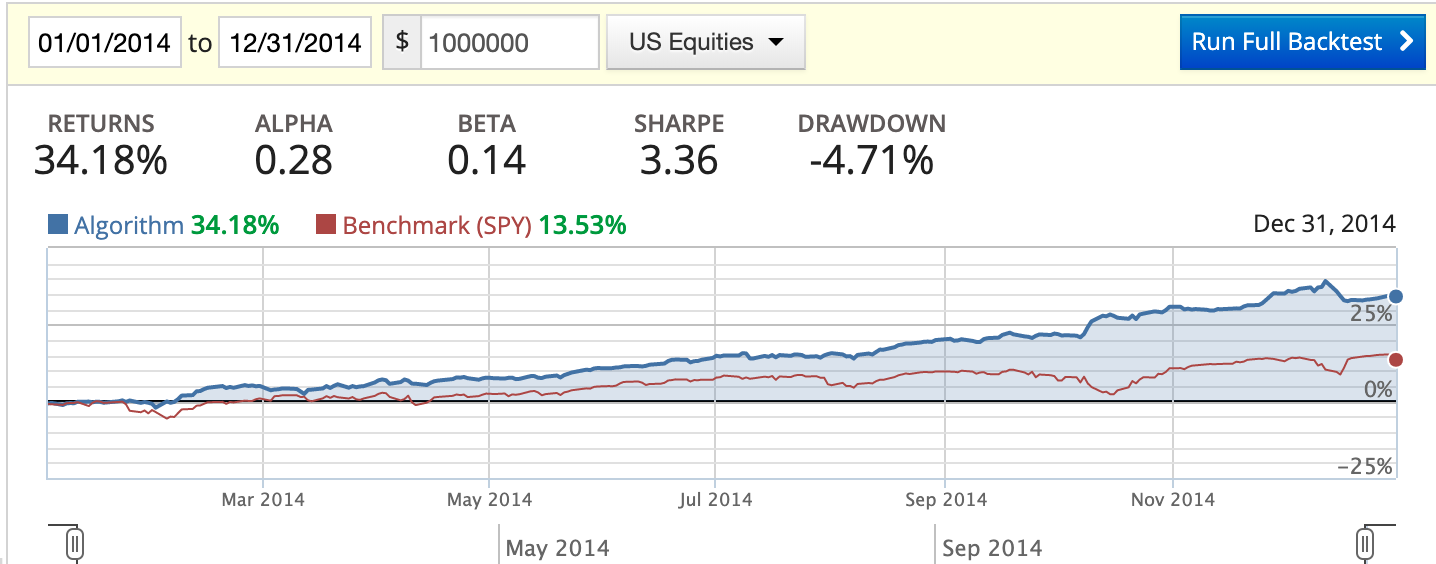
\includegraphics[scale=0.5,bb=0 0 640 480]{figures/mad_mfd_macd_2014.png}
\caption{Comparison of proposed algorithm to SPY; 2014.}
\label{fig:backtest-2014}
\end{figure}

\begin{figure}
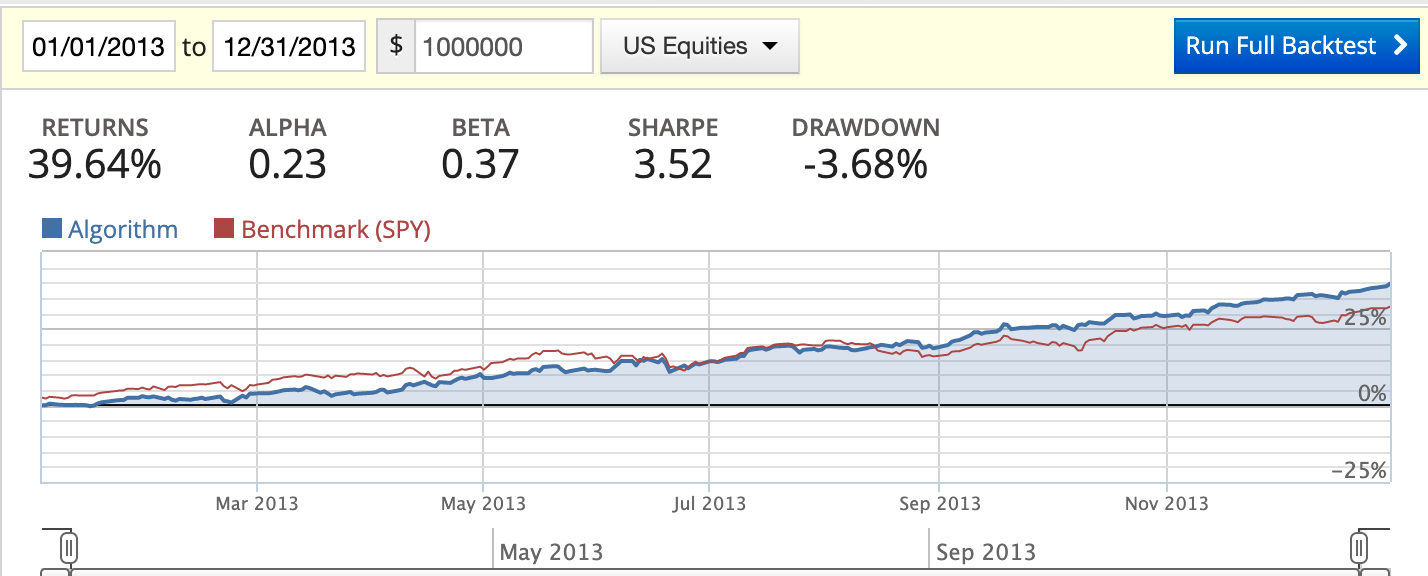
\includegraphics[scale=0.5,bb=0 0 640 480]{figures/mad_mfd_macd_2013.png}
\caption{Comparison of proposed algorithm to SPY; 2013.}
\label{fig:backtest-2013}
\end{figure}

\begin{figure}
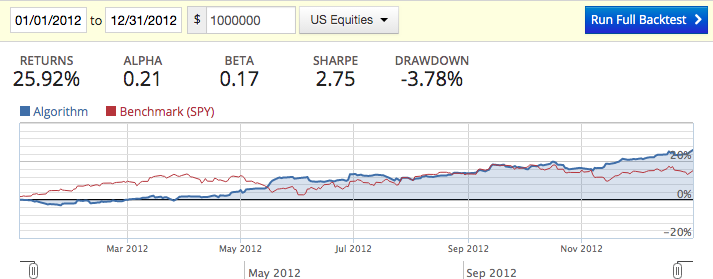
\includegraphics[scale=0.5,bb=0 0 640 480]{figures/mad_mfd_macd_2012.png}
\caption{Comparison of proposed algorithm to SPY; 2012.}
\label{fig:backtest-2012}
\end{figure}

\begin{figure}
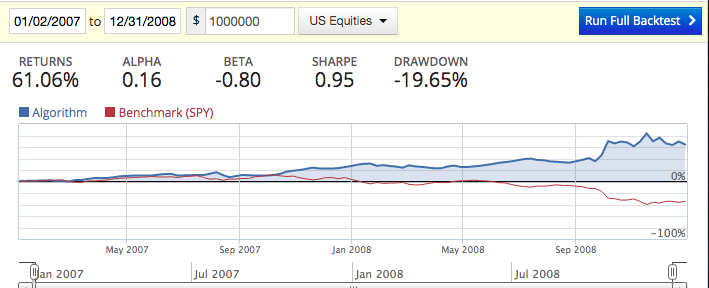
\includegraphics[scale=0.5,bb=0 0 640 480]{figures/crash_period_mfd_macd.png}
\caption{Comparison of proposed algorithm to SPY; 2007-2008.}
\label{fig:backtest-2007-2008}
\end{figure}

\begin{figure}
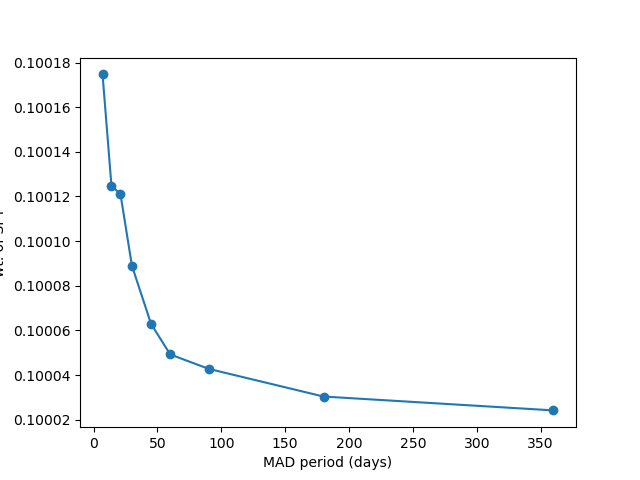
\includegraphics[scale=0.9,bb=0 0 640 480]{figures/mad-sensitivity-period-SPY.png}
\caption{The weight of SPY vs. period used for calculation of MAD.}
\label{fig:mad-period-sensitivity}
\end{figure}

\clearpage

\bibliography{references}
\bibliographystyle{plain}

\end{document}

